\section{Bosonic $SU(M)$ coherent states}
	
\subsection{Construction}
In this subsection, I describe the properties of $SU(M)$ coherent states constructed on bosonic annihilation and creation operators.

While I use a slightly different ansatz than the one in (\cite{grossmann,buonsante}) regarding the construction of bosonic $SU(M)$ coherent states, the difference is minor (I do not impose an extra condition on the components of the CS parameter $z$, and include an explicit normalisation factor instead). The ansatz I use is the same as the one used by Grigolo, Viscondi, and de Aguiar in \cite{sampling_algorithm}. Therefore the content of this subsection is not to be considered original work by me, and is instead a continuation of the literature review in the previous chapter. It is included in this chapter, however, to draw contrast with the fermionic $SU(M)$ coherent states, whose construction does contain original work by me (namely, the operator sequence matrix elements).

\subsubsection{Reference state and displacement operator}
A suitable reference state for a bosonic system of $M$ modes and $S$ particles is
\begin{equation}
\ket{\phi_0}=\ket{0,0\dots 0, S}
\end{equation}
Finding the stability subgroup of the dynamical group for this reference state, we ultimately obtain the displacement operator
\begin{equation}
\hat{D}(z)=\exp(\sum_{i=1}^{M-1}z_i\hat{b}\hc_i\hat{b}_M)
\end{equation}
The bosonic $SU(M)$ coherent state is then
\begin{equation}
\ket{z}=N(z)\exp(\sum_{i=1}^{M-1}z_i\hat{b}\hc_i\hat{b}_M)\ket{\phi_0}
\end{equation}
where $z$ is a vector of $M-1$ complex parameters

\subsubsection{Decomposition into the occupancy basis}
As shown by Buonsante and Penna in \cite{buonsante}, this coherent state can be decomposed into the occupancy basis as follows:
\begin{equation} \label{eq:bosonic_decomposition}
\ket{\vec{z}}=\frac{N(z)}{\sqrt{S!}}\left(\hat{a}^\dagger_M+\sum_i^{M-1}z_i\hat{a}^\dagger_i\right)^S\ket{0,0\dots 0}
\end{equation}
This result can be obtained by following the method outlined in Sec. \ref{sec:general_decomposition}. Applying the multinomial theorem gives the explicit superposition of occupancy basis states equivalent to the coherent state:
\begin{equation}
\ket{z}=N(z)\sum_{k_1+k_1+\dots +k_M=S}\sqrt{\frac{S!}{k_1!k_2!\dots k_M!}}z_1^{k_1}z_2^{k_2}\dots z_{M-1}^{k_{M-1}}\ket{k_1,k_2\dots k_M}
\end{equation}

\subsubsection{Overlap and normalisation}
Using Eq. \ref{eq:bosonic_decomposition} and Wick's theorem, the overlap of two bosonic CSs can be shown \cite{grossmann} to be
\begin{equation} \label{eq:bosonic_overlap}
\braket{z_a}{z_b}=N(z_a)N(z_b)\left(1+\sum_i^{M-1}z_{a,i}^*z_{b,i}\right)^S
\end{equation}
This also determines the normalisation function as
$N(z)=\left(1+\sum z_i^*z_i\right)^{-\frac{S}{2}}$


\subsubsection{Matrix element of bosonic operator sequences}
Consider a normal-ordered product sequence of $x$ bosonic creation and $x$ bosonic annihilation operators. Its matrix element for two arbitrary CSs can be shown \cite{grossmann} to be
\begin{equation} \label{eq:bosonic_OSME}
\mel{z_a}{\hat{b}\hc_{\rho_1}\dots\hat{b}\hc_{\rho_x}\hat{b}_{\sigma_1}\dots\hat{b}_{\sigma_x}}{z_b}=z_{a,\rho_1}^*\dots z_{a,\rho_x}^*z_{b,\sigma_1}\dots z_{b,\sigma_x} \braket{z_a^{(x)}}{z_b^{(x)}}
\end{equation}
where the \textit{reduced overlap} is defined as
\begin{equation}
\braket{z_a^{(x)}}{z_b^{(x)}}=N(z_a)N(z_b)\left(1+\sum_i^{M-1}z_{a,i}^*z_{b,i}\right)^{S-x}
\end{equation}
i.e. the reduced unnormalised CSs behave as if their associated total particle number was reduced by $x$.

This is an important mathematical property to know in our methodology, as in the equations of motion operator sequences up to the third order are present (the partial derivatives of Hamiltonian matrix elements).

\subsection{Time complexity of evaluation}
Using standard techniques, the evaluation of the overlap in Eq. \ref{eq:bosonic_overlap} has time complexity $O(M)$, as does the evaluation of the bosonic operator sequence matrix element in Eq. \ref{eq:bosonic_OSME}. Given a second-order Hamiltonian, its matrix element for two states $\ket{z_a},\ket{z_b}$ may be evaluated with time complexity $O(M^5)$, and the full Hamiltonian matrix with time complexity $O(M^5N^2)$ for a sample basis of $N$ coherent states. The dynamical matrix $\Omega$ in Eq. \ref{eq:dynamical_matrix} has dimensions $(MN\cross MN)$, it may be evaluated in $O(M^3N^2)$, and inverted in $O(M^3N^3)$. Therefore the main bottlenecks are evaluating the Hamiltonian matrix (for large $M$) and inverting the dynamical matrix (for large $N$). However, in the case of the Bose-Hubbard model, the time complexity of evaluating the Hamiltonian matrix is lowered by a factor of $M^2$, as it is in tridiagonal form.


\subsection{Results}
The method proposed by us in Sec. \ref{sec:bosonic1} has been implemented and tested on the Bose-Hubbard model with the results by Qiao and Grossmann as a benchmark.

Qiao and Grossmann tested their fully variational method on a two-mode and a three-mode system of $50$ particles, with the initial wavestate being a pure coherent state.

In the following figures, the "true" solution is obtained by explicit propagation on the full occupancy basis unless stated otherwise.

The particular Hamiltonian parameters in these results match the ones chosen by Qiao and Grossmann in \cite{grossmann}.

\subsubsection{Initial wavestate as a pure coherent state}
When the initial wavestate is set to be a pure coherent state, our method becomes a massive improvement, since the trajectory of a single coherent state is semi-classical, and we can find it with a basis sample of size $N=1$. In Fig. \ref{fig:single_peak_benchmark} I show the convergence of this minimal basis sample to the true solution for both two-mode and three-mode systems.

\begin{figure} \label{fig:single_peak_benchmark}
\begin{center}
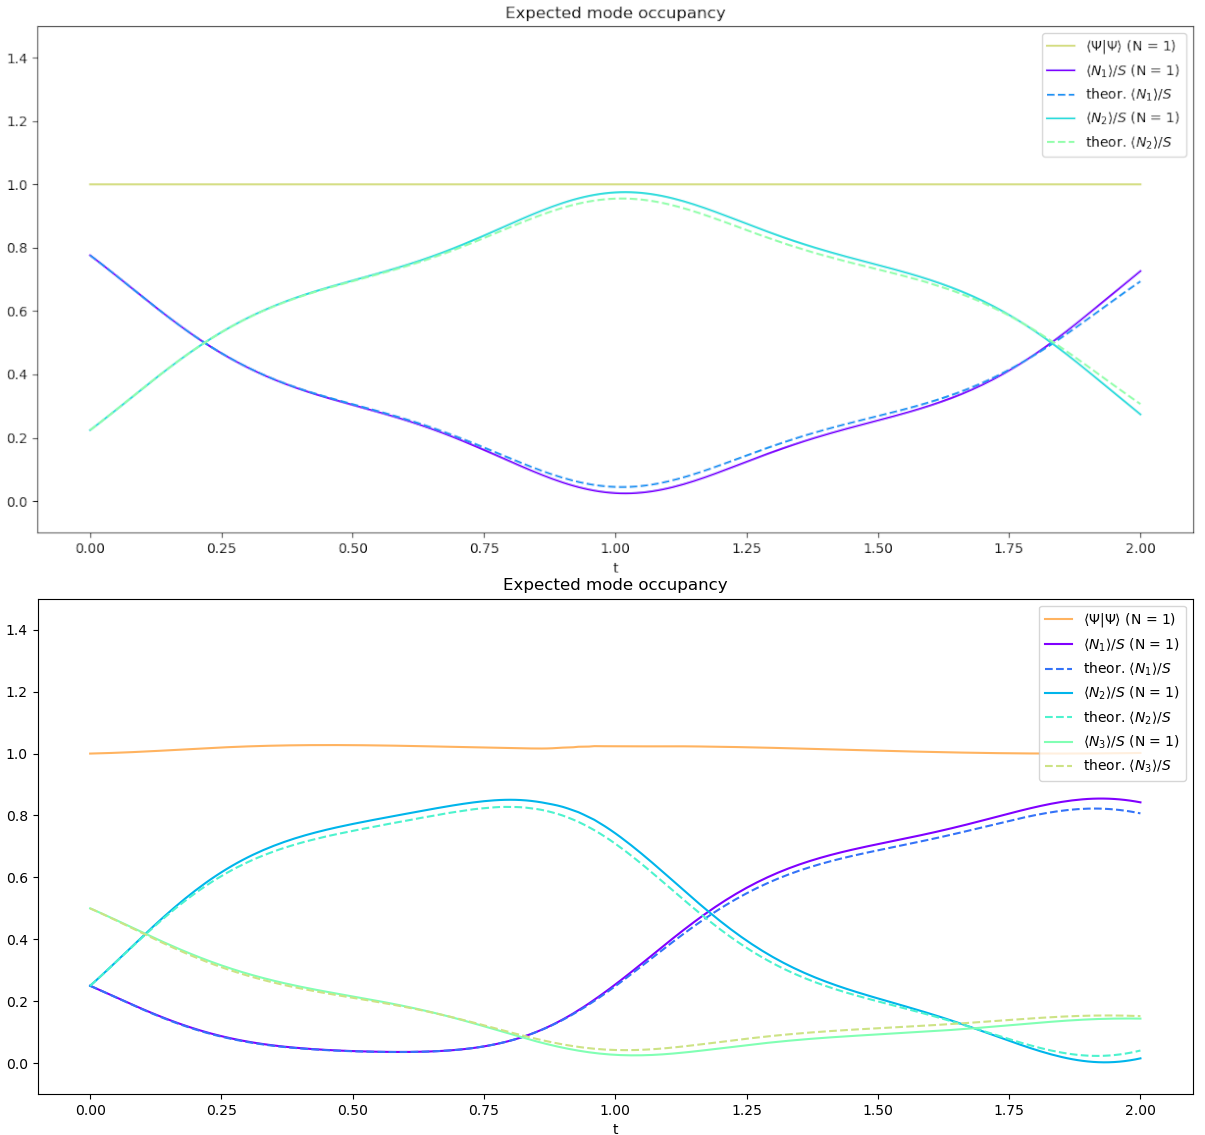
\includegraphics[width=\textwidth]{images/single_peak_benchmark}
\caption{These graphs show the calculated trajectories of bosonic pure coherent states using the single CS equations of motion as compared to the decomposition onto the full occupancy basis. Both trajectories are calculated using the Dormand-Prince method. The top graph shows a system with $M=2,S=20$ and the bottom graph shows a system with $M=3,S=20$. We see convergence for both the two-mode and the three-mode system, although the three-mode system is slightly less numerically stable (notice the wiggle in the total wavefunction norm). The CS solution is obtained in the order of $100$ ms; for the two-mode system, the full occupancy solution is obtained in the order of $1$ s; for the three-mode system, the full occupancy solution is obtained in the order of $1$ h.}
\end{center}
\end{figure}

\subsubsection{Initial wavestate as a superposition of coherent states}
We wish to show that the propagation of each basis state separately yields a suitable time-dependent frozen basis for an arbitrary initial wavefunction. Therefore I extended the pool of initial wavestates to superpositions of a small number of coherent states, and chose the basis for each setup as a set of all present coherent states. Fig. \ref{fig:multiple_peaks_benchmark} demonstrates the validity and scope of this approach.

\begin{figure} \label{fig:multiple_peaks_benchmark}
\begin{center}
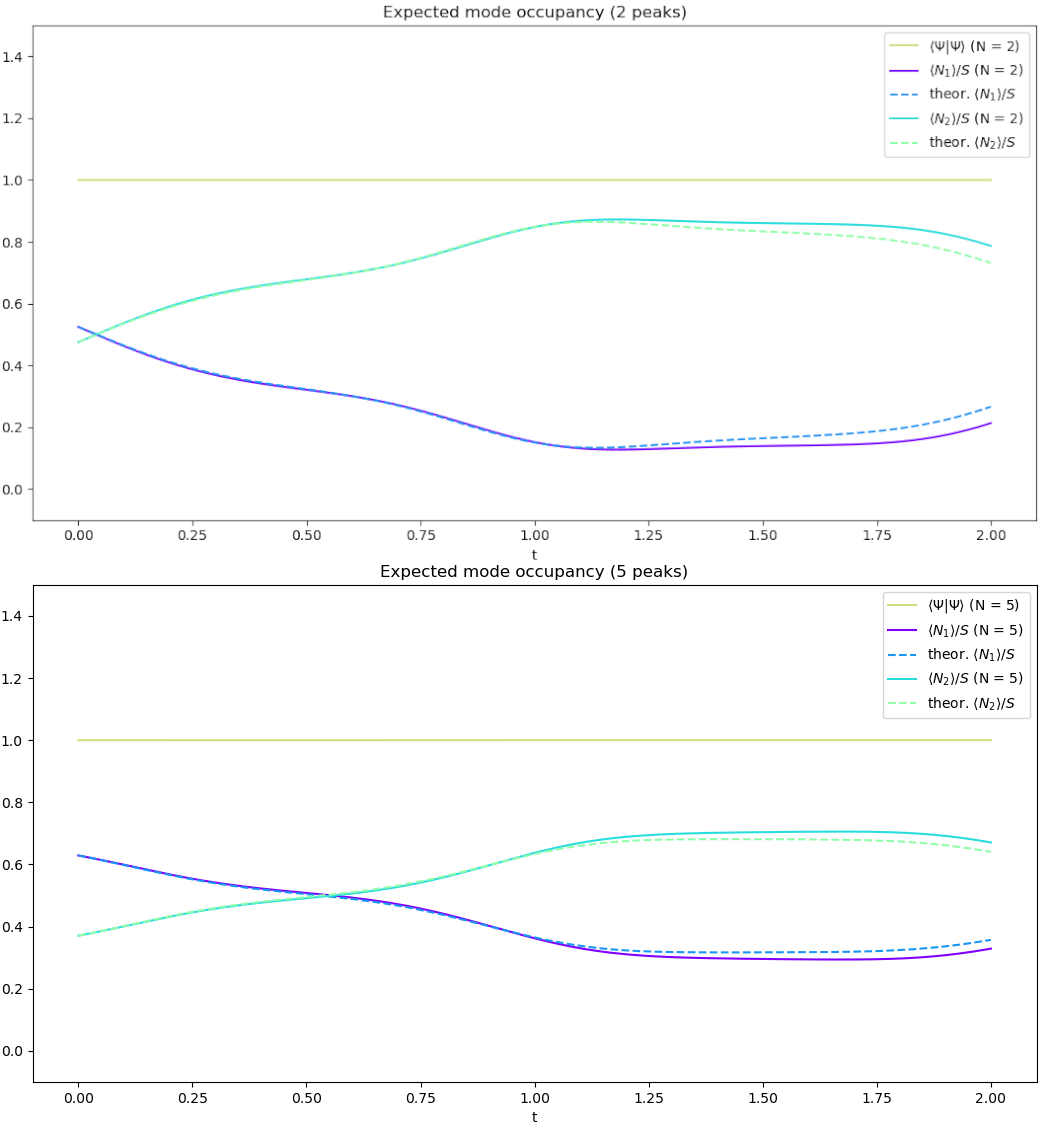
\includegraphics[width=\textwidth]{images/multiple_peaks_benchmark}
\caption{These graphs both show the evolution on a two-mode system with $S=20$; the upper graph has the initial wavefunction a superposition of $2$ pure coherent states, and the bottom graph a superposition of $5$ pure coherent states. For both graphs, the basis is chosen to be equal to the components of the initial wavefunction superposition, and the evolution converges to the true solution. Choosing an initial wavefunction a superposition of a larger number of coherent states (say $20$) will, however, prevent the model from converging easily, which shows the limit of this naive sampling method. For such highly-mixed initial wavefunctions, more general sampling methods are required (such as magnitude-squared weighted sampling from the parameter space). Nevertheless, this shows the validity of our method beyond pure-CS initial wavefunctions, extending it beyond the scope on which Qiao and Grossmann demonstrated their fully variational method.}
\end{center}
\end{figure}